\capitulo{1}{Introducción}

Los sistemas embebidos o empotrados (SE) están muy presentes en nuestra vida cotidiana \cite{UnicanSE}. Algunos ejemplos de sistemas empotrados que podemos encontrar en nuestro día a día serían los electrodomésticos, relojes, coches, semáforos, entre otros. Todos estos aparatos, junto con robots o máquinas industriales, componen un campo importante para nuestra sociedad, ya que estos sistemas facilitan enormemente tareas pesadas o repetitivas en la vida de las personas.

Podemos referirnos a estos sistemas como un microcontrolador. Es importante conocer las diferencias entre un microcontrolador y un microcomputador \cite{ALMCMP}. Como diferencias a nivel técnico tenemos:
 
\begin{itemize}
\item En lo referido al software, encontramos que los microcontroladores tienen como objetivo la realización de pequeñas tareas programadas por un desarrollador para un fin concreto. Es por ello que cuentan con algunas características a nivel general de todos los microcontroladores como puede ser, bajo consumo, tamaño reducido y bajo coste. En cambio, un microcomputador se suele utilizar para entornos complejos y tareas extensas que a su vez requieren de otras tareas en cascada.
\item A nivel de hardware, encontramos que un microcontrolador engloba tanto la unidad de procesamiento como una pequeña unidad de memoria (ROM, RAM, etc), además de algunos puertos para periféricos, un temporizador, etc. Podemos pensar en un microcontrolador como una minicomputadora.
\end{itemize}

En cuanto a los periféricos, se les pueden añadir sensores dotándoles de nuevas funcionalidades como por ejemplo, medición de humedad y calor, envío y recibo de ultrasonidos y comunicaciones bluetooth o infrarroja y un largo etc.  

Para que todos estos dispositivos puedan funcionar adecuadamente, se necesitan o al menos se prefiere tener a estos sistemas conectados entre sí. Mediante la transferencia de datos se pueden implementar aún más procesos, siempre con el objetivo de ser más eficiente a la hora de solucionar un problema.

Ahora que ya hemos visto su importancia y uso en la actualidad, veamos cómo funcionan los sistemas empotrados en tiempo real. En la mayoría de los casos en los que se utilizan sistemas embebidos, se requiere que realicen las operaciones rápidamente. Una instrucción debe ser ejecutada de manera inmediata o con un retardo mínimo. Para conseguirlo se suelen utilizar Sistemas Operativos en Tiempo Real (RTOS) para la gestión del tiempo de ejecución de cada tarea.

 Los SE son parte central de este nuevo mundo interconectado, en el cual todos nuestros aparatos electrónicos se comunican entre ellos mediante un hardware específico y un software que cumple con tareas en tiempo real. Esta tecnología cada vez está más presente en nuestros hogares y sin duda es un gran avance hacia el bienestar de las personas.


\section{Descripción del trabajo realizado}\label{sec:Descripcion}

La idea principal de este proyecto es disponer de varios sistemas embebidos conectados en red, que se comuniquen mediante cable ethernet. Esta conexión será de tipo punto a punto. Dispondremos de tres placas FRDM-K64F. A una de ellas se le añadirá además un \extranjerismo{shield} de expansión que la dotará de más periféricos, de las cuales usaremos los 4 botones, las 4 luces led de cara a la interacción con el usuario, además de los dos potenciómetros y el sensor de temperatura. 
En el caso de las otras dos placas, disponen de una pantalla LCD y además están conectadas a una placa controladora de dos motores EMG30. 

La Figura \ref{esqCon} muestra el diagrama de conexiones para ver cómo está construida, la planta piloto.

%\imagen{esquemaLaboratorio}{Esquema de conexiones del Laboratorio}\label{esqCon}
\begin{figure}[!h]
	\centering
	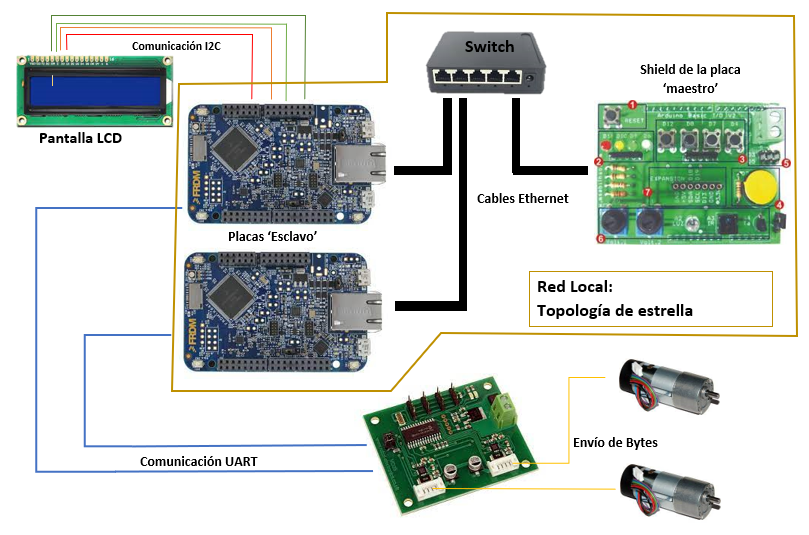
\includegraphics[width=0.9\textwidth]{esquemaLaboratorio}
	\caption{Esquema de conexiones del laboratorio.}\label{esqCon}
\end{figure}

Como podemos observar, la planta piloto consta de una red local cableada de tipo ethernet. La red está compuesta por tres sistemas empotrados conectados entre sí mediante un switch a través de cable ethernet, siguiendo una topología de estrella. La comunicación se realiza terminal a terminal, pasando por un switch, que reenvía los paquetes enviados de forma que lleguen correctamente a su destinatario.
La placa de color verde que vemos en la imagen anterior es el shield de expansión que está colocado encima de la placa maestro. El shield contiene los dos potenciómetros, 4 botones, 4 leds y el sensor de temperatura con los que se interactuará con el resto de los sistemas embebidos.
Por último, la Figura \ref{PlantaPiloto} muestra la planta piloto.

%\imagen{proyecto}{Planta piloto del proyecto.}\label{PlantaPiloto}
\begin{figure}[!h]
	\centering
	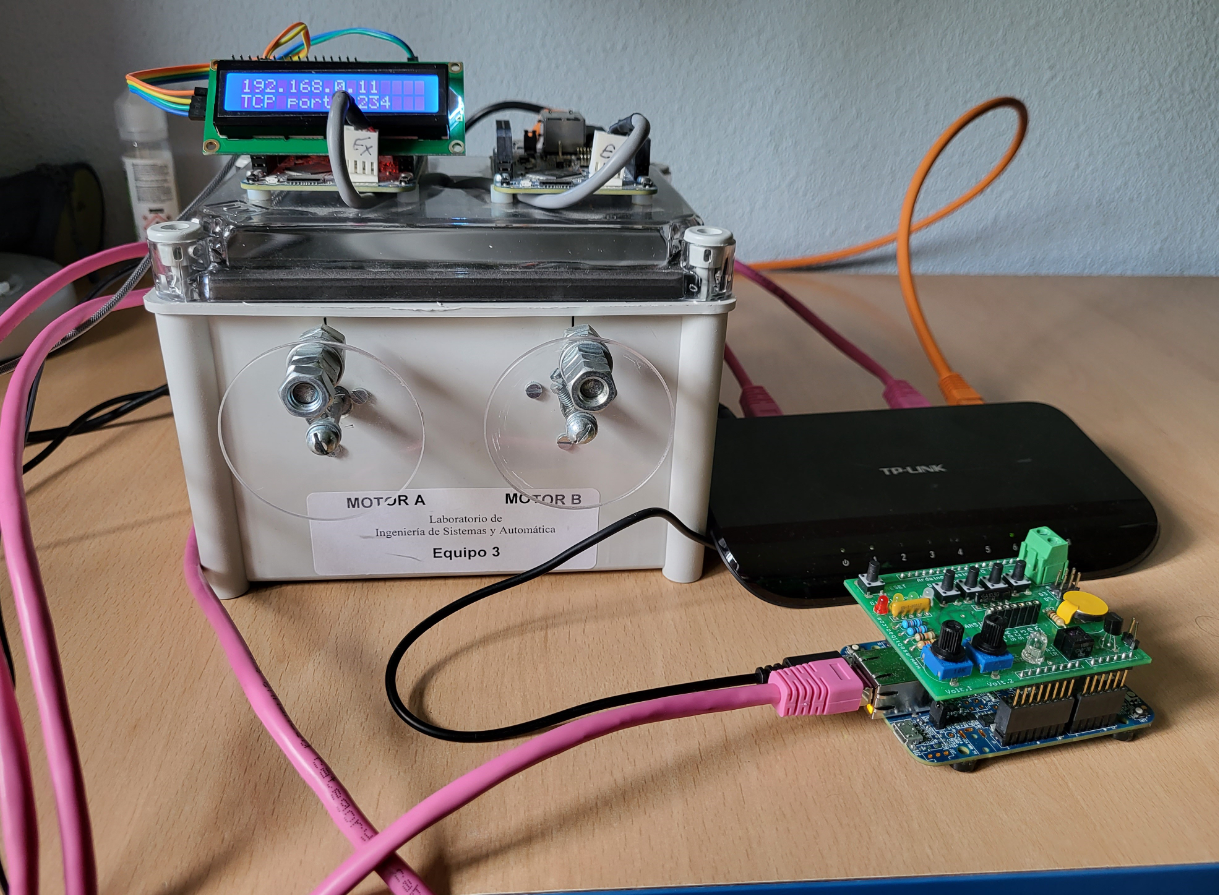
\includegraphics[width=0.9\textwidth]{proyecto}
	\caption{Planta piloto del proyecto.}\label{PlantaPiloto}
\end{figure}

El funcionamiento consta de los siguientes casos de uso:
\begin{itemize}
\item Mediante el potenciómetro 1 fijaremos la velocidad y sentido del giro del motor A. Una vez regulado enviaremos la petición pulsando el botón 1.
\item El potenciómetro 2 y el botón 2 se utilizan de la misma manera para fijar la velocidad del motor B.
\item El botón 3 nos sirve como parada de emergencia para los dos motores.
\item Al pulsar el botón 4 la placa maestro reporta la temperatura captada por el sensor de temperatura y se muestra por pantalla.
\item El botón 5 y 6 realizan una petición a la placa controladora de los motores para saber a qué velocidad giran el motor A y el motor B respectivamente.
\end{itemize}

\section{Estructura de la memoria}\label{sec:Estructura}

La memoria de este proyecto está estructurada de la siguiente manera.

\begin{description}
	\item[Introducción.] Se explican los temas principales en los que se basa tanto la idea como el procedimiento y funcionalidad final del proyecto.

	\item[Objetivos del proyecto.] Se explican los objetivos del proyecto tanto generales, como técnicos y personales, que se esperan cumplir durante la realización del proyecto.

	\item[Conceptos teóricos.] Se tratan los conceptos teóricos más detalladamente. Conceptos como el protocolo TCP/IP, las conexiones en red y comunicaciones con otros periféricos.

	\item[Técnicas y herramientas.] En este apartado se verán las herramientas utilizadas para llevar a cabo este proyecto, así como las técnicas para la correcta organización y gestión del trabajo.

	\item[Aspectos Relevantes del desarrollo.] En este capítulo se mostrarán algunos conceptos e hitos importantes durante el desarrollo del trabajo.

	\item[Trabajos relacionados.] Se mostrarán algunos ejemplos de uso real en la actualidad, que utilizan sistemas empotrados para su desarrollo

	\item[Conclusiones y líneas de trabajo futuras.] Se mencionarán algunas propuestas sobre hacia donde podría evolucionar el trabajo expuesto en esta memoria y a que conclusiones se ha llegado tras haber completado el objetivo del trabajo.
\end{description}

\section{Anexos}\label{sec:anexos}
Los anexos consisten en:
\begin{description}
	\item[Plan del proyecto software.] Se muestra la planificación temporal y la viabilidad del proyecto dividida en dos partes, legal y económica.

	\item[Especificación de requisitos del software.] Se expone un catálogo de requisitos para la utilización de este sistema en un entorno real. Este catálogo viene con la definición de cada una de sus partes.

	\item[Especificación de diseño.] Exposición de la fase de diseño, el plan procedimental y el diseño arquitectónico de las placas y sensores que componen el sistema.

	\item[Manual del programador.] Explicación de aquellos conocimientos e ideas que un programador debería conocer para poder entender y seguir desarrollando el código fuente.

	\item[Manual de usuario.] Contiene una explicación sobre el debido uso y pasos a seguir para que un usuario pueda utilizar adecuadamente el software.
\end{description}

\section{Contenido adjunto}\label{sec:Contenido adjunto}
\begin{enumerate}
\item Software para las placas `Shield' y `Placa motor A' y `Placa motor B'.
\item Video del funcionamiento de la planta piloto compuesta por dos motores y su placa controladora, una pantalla LCD, tres placas k64f y una placa de expansión.
\item Repositorio de GitHub \cite{EOD1001} con todo el contenido de desarrollado.
\item Software documentado.
\end{enumerate}

